\chapter{Gestión del proyecto}
La gestión de proyectos de software es una parte esencial de la ingeniería del software. La buena gestión no puede garantizar el éxito del proyecto. Sin embargo, la mala gestión normalmente lleva al fracaso del proyecto. La gestión del proyecto es una etapa llevada a cabo a lo largo de todo el ciclo de vida del proyecto como método para lograr que el producto final se ajuste a las necesidades y restricciones impuestas (tiempo, costes, requerimientos, etc.).

En este capítulo se realiza la gestión de costes del proyecto, donde se detalla el análisis de riesgos, la metodología de desarrollo empleada,  la gestión de configuración, la planificación temporal y la estimación de costes del proyecto.

\section{Análisis de riesgos} \label{riesgos}
Una tarea importante del gestor de proyectos es anticipar los riesgos que podrían afectar a la programación del proyecto o a la calidad del software a desarrollar y emprender acciones para evitar esos riesgos.

Un riesgo de un proyecto es un evento o condición incierto que, si se produce, tendrá un efecto positivo o negativo sobre al menos un objetivo del proyecto, como tiempo, coste, alcance o calidad, es decir, cuando el objetivo de tiempo de un proyecto es cumplir con el cronograma acordado; cuando el objetivo de coste del proyecto es cumplir con el coste acordado, etc. 

El riesgo está compuesto de tres componentes esenciales:
\begin{itemize}
\item Un evento definible.
\item Probabilidad de ocurrencia.
\item Consecuencia de la ocurrencia (impacto).
\end{itemize}

En este proyecto, se consideran los riesgos que, en caso de producirse, tendrían un efecto negativo sobre el proyecto.

En las metodologías ágiles y en concreto en Scrum, que es la metodología utilizada en este proyecto (explicada en \ref{scrum}), los ciclos de desarrollo son cortos, se hacen constantes revisiones y se considera la idea de incertidumbre desde el principio (de la que tienen origen normalmente los riesgos). Scrum se encarga del riesgo a principios del ciclo de vida del proyecto y sustituye la gestión del riesgo explicita (la gestión de riesgos utilizada en las metodologías tradicionales, donde la burocracia dificulta que se lleve a cabo la disciplina y actualización adecuada) por la gestión del riesgo continua. Esta gestión continua es realizada en las distintas reuniones que se llevan a cabo a lo largo del desarrollo del proyecto.
%En estas reuniones, las personas relacionadas con el proyecto se hacen preguntas como: ¿Qué impedimentos hemos encontrado?. Responder a este tipo de preguntas periódicamente es una forma implícita de gestionar los riesgos del proyecto. En las reuniones donde interviene el cliente, por ejemplo, se pueden detectar y atajar todos los riesgos relacionados con la comunicación con éste y los requisitos. Para que funcione esta forma de gestionar los riesgos, se debe hacer hincapié en que no sólo se hable de los impedimentos actuales sino de también de los futuros.

A continuación, se enumeran los posibles riesgos en dos grupos. Para ello, se identifica el riesgo, se da una breve descripción, se analiza (cuál sería la probabilidad y el impacto) y se indican posibles estrategias de prevención, minimización o contingencia. Esta descripción está basada en la gestión de riesgos propuesta por el ingeniero de software Ian Sommerville en su libro \cite{sommerville}.

\noindent
\textbf{Riesgos del proyecto:} Afectan a la calendarización o los recursos.

%Riesgo proyecto 1
\begin{table}[H]
	\begin{tabular}{| p{4cm}| p{10cm} |}
		\hline
		\multicolumn{2}{|c|}{\textbf{RPY-1} - Retraso respecto a la planificación temporal} \\ \hline
		\textbf{Descripción:} & No se consigue seguir la planificación prevista debido a una mala organización, planificación o debido a que tiene lugar algún otro riesgo descrito a continuación. \\ \hline
		\textbf{Probabilidad:} & Alta \\ \hline
		\textbf{Impacto:} & Serio \\ \hline
		\textbf{Estrategia de prevención:} & Las reuniones de planificación y revisión de los incrementos (sprints) con los directores del proyecto llevadas a cabo en la metodología Scrum sirven de estrategia de prevención, ya que se puede validar el progreso. \\ \hline
		\textbf{Plan de contingencia:} & Ajustar la planificación inicial. \\ \hline
	\end{tabular}
\end{table}

\noindent
\textbf{Riesgos del producto:} Afectan a la calidad o al rendimiento del software.

%Riesgo producto 1
\begin{table}[H]
	\begin{tabular}{| p{4cm}| p{10cm} |}
		\hline
		\multicolumn{2}{|c|}{\textbf{RPD-1} - Alteración de los requisitos} \\ \hline
		\textbf{Descripción:} & No se definen todos los requisitos al inicio del desarrollo o algunos requisitos cambian debido por ejemplo a que una prueba de hipótesis no devuelve los resultados esperados o no existe suficiente información para llevar a cabo su implementación. \\ \hline
		\textbf{Probabilidad:} & Moderada \\ \hline
		\textbf{Impacto:} & Tolerable \\ \hline
		\textbf{Estrategia de minimización:} & La metodología Scrum utilizada en este proyecto asume la incertidumbre y por tanto considera que los requisitos pueden cambiar a lo largo del desarrollo, con lo cual constituye una forma de minimizar el impacto. \\ \hline
	\end{tabular}
\end{table}

%Riesgo producto 2
\begin{table}[H]
	\begin{tabular}{| p{4cm}| p{10cm} |}
		\hline
		\multicolumn{2}{|c|}{\textbf{RPD-2} - Escasa información de un determinado test estadístico} \\ \hline
		\textbf{Descripción:} & La información existente de una determinada prueba de hipótesis es escasa, debido a que el test es reciente y aún no existe mucha documentación, lo que dificulta e impide que se pueda implementar de forma correcta. \\ \hline
		\textbf{Probabilidad:} & Baja \\ \hline
		\textbf{Impacto:} & Tolerable \\ \hline
		\textbf{Estrategia de prevención:} & Buscar información en artículos relacionados con el autor o tests similares que puedan ayudar a entender qué operaciones realiza el test. \\ \hline
		\textbf{Plan de contingencia:} & Sustituir el test estadístico por otro de similares características para el que sí haya documentación. \\ \hline
	\end{tabular}
\end{table}

%Riesgo producto 3
\begin{table}[H]
	\begin{tabular}{| p{4cm}| p{10cm} |}
		\hline
		\multicolumn{2}{|c|}{\textbf{RPD-3} - Resultados test no esperados} \\ \hline
		\textbf{Descripción:} & Los resultados obtenidos de la aplicación de un test no son los esperados. Cabe destacar que puede que para un determinado conjunto de datos de entrada los resultados obtenidos sean mejores que los resultados obtenidos para otros datos. \\ \hline
		\textbf{Probabilidad:} & Moderada \\ \hline
		\textbf{Impacto:} & Tolerable \\ \hline
		\textbf{Estrategia de prevención:} & Programar paso a paso contrastando los resultados de se obtienen y probar con diferentes conjuntos de datos. \\ \hline
		\textbf{Plan de contingencia:} & Sustituir el test estadístico por otro de similares características que funcione mejor. \\ \hline
	\end{tabular}
\end{table}

%Riesgo producto 4
\begin{table}[H]
	\begin{tabular}{| p{4cm}| p{10cm} |}
		\hline
		\multicolumn{2}{|c|}{\textbf{RPD-4} - Mala usabilidad de la plataforma} \\ \hline
		\textbf{Descripción:} & La web no es lo suficientemente clara y fácil de usar para los usuarios finales. \\ \hline
		\textbf{Probabilidad:} & Baja \\ \hline
		\textbf{Impacto:} & Serio \\ \hline
		\textbf{Estrategia de prevención:} & Las reuniones de revisión de los incrementos (sprints) con los directores del proyecto (``representantes" de la voz del cliente) llevadas a cabo en la metodología Scrum sirven de estrategia de prevención, haciendo que la probabilidad de ocurrencia de este riesgo sea mínima. \\ \hline
		\textbf{Plan de contingencia:} & Establecer una reunión urgente con los directores para tratar de determinar las causas y reconstruir las características que fallan. \\ \hline
	\end{tabular}
\end{table}

\section{Metodología de desarrollo} \label{metodologia}

\subsection{Metodologías ágiles}
En todo proyecto software la elección de la metodología de desarrollo juega un papel crucial a la hora de finalizar con éxito el proyecto. El diseño y el desarrollo de software no es una tarea sencilla y cada proyecto tiene características personales que propician la selección de una determinada metodología u otra.

Al principio, cuando el desarrollo de software todavía se estaba iniciando, surgió la necesidad de mejorar el proceso para poder finalizar con éxito los proyectos, con lo que se implantaron y adaptaron metodologías existentes en otras áreas al desarrollo de software. Estas metodologías tradicionales o también denominadas pesadas dividen el proceso de desarrollo en varias etapas que se van realizando de manera secuencial, siendo la primera fase aquella que sienta las bases del proyecto. Uno de los principales inconvenientes que tienen estas metodologías es su baja tolerancia a los cambios, así como el no ofrecer una buena solución en entornos volátiles.

En un escenario rápido e inestable, encajan mal las estrategias de negocio predictivas (metodologías pesadas), que diseñan un producto y trazan un plan de negocio. Es en este ámbito donde surgen las metodologías ágiles, que ofrecen una mayor libertad al equipo de trabajo cuando existe incertidumbre. No se trata de elegir un modelo como el mejor, simplemente habrá casos en los que convendrá una gestión predictiva (p.ej. cuando los requisitos están completamente determinados desde el principio y no habrá cambios) y otros (p.ej. entornos volátiles) en los que la opción ágil puede ser más beneficiosa.

En marzo de 2001, 17 críticos de los modelos de producción basados en procesos, convocados por Kent Beck, que había publicado un par de años antes el libro en el que explicaba la nueva metodología Extreme Programming Beck \cite{kent}) se reunieron en Salt Lake City para discutir sobre el desarrollo de software. En la reunión se acuñó el término ``Métodos Ágiles" para definir a aquellos que estaban surgiendo como alternativa a las metodologías formales, a las que consideraban excesivamente pesadas y rígidas por su carácter normativo y fuerte dependencia de planificaciones detalladas, previas al desarrollo. Los integrantes de la reunión resumieron en cuatro postulados lo que ha quedado denominado como ``Manifiesto Ágil", que son los valores sobre los que se asientan estos métodos:

\begin{itemize}
\item Se valora más a los individuos y su interacción que a los procesos y las herramientas.
\item Se valora más el software que funciona que la documentación exhaustiva.
\item Se valora más la colaboración con el cliente que la negociación contractual.
\item Se valora más la respuesta al cambio que el seguimiento de un plan.
\end{itemize}

\noindent
Sobre estos valores, se establecen una serie de principios de las metodologías ágiles, como son:

\begin{itemize}
\item Requisitos cambiantes bienvenidos.
\item Potenciar las conversaciones en persona.
\item Producto funcional como medida de progreso.
\item Satisfacer al cliente mediante entregas tempranas.
\end{itemize}

\begin{figure}[t!]
\centering
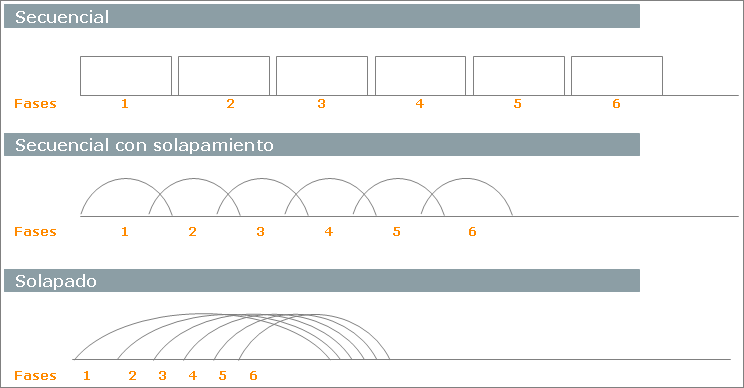
\includegraphics[width=12cm,height=6cm]{figuras/ciclos_desarrollo.png}
\caption{Ciclos de desarrollo.}
\label{fig:ciclos}
\end{figure}

\subsection{Scrum} \label{scrum}
Existen muchas metodologías ágiles disponibles, como el método de desarrollo de sistemas dinámicos (DSDM), la programación extrema (XP), etc. Sin embargo, en este proyecto se hace uso de la metodología Scrum. Actualmente, Scrum es una de las metodologías más populares para la gestión de proyectos. Este modelo fue identificado y definido por Ikujiro Nonaka e Hirotaka Takeuchi a principios de los 80, al analizar cómo desarrollaban los nuevos productos las principales empresas de manufactura tecnológica en esa época. Nonaka y Takeuchi compararon la nueva forma de trabajo en equipo, con el avance en formación de scrum de los jugadores de Rugby, a raíz de lo cual quedó acuñado el término “scrum” para referirse a ella.

Entre las características que describen los entornos de desarrollo típicos en los que se puede aplicar la metodología de desarrollo ágil Scrum, destacan las siguientes:

\begin{itemize}
\item La incertidumbre: Es asumida en el desarrollo del proyecto, en donde se apunta cuál es la visión genérica que se quiere conseguir, o la dirección estratégica que hay que seguir, pero no un plan detallado del producto y su desarrollo (para lo cual se da un margen de libertad).
\item Fases del desarrollo solapadas: Las fases no existen como tal sino que se desarrollan tareas/actividades en función de las necesidades cambiantes durante todo el proyecto. De hecho, en muchas ocasiones no es posible realizar un diseño técnico detallado antes de empezar a desarrollar y ver algunos resultados. En la figura \ref{fig:ciclos}, podemos ver gráficamente en el tercer caso el solapamiento de fases, mientras que en el primer caso el retraso en una fase hace de cuello de botella en el proyecto. El solapamiento diluye el ruido y los problemas entre fases.
\item Control sutil: El equipo trabaja con autonomía en un entorno de ambigüedad, inestabilidad y tensión. La gestión establece puntos de control suficientes para evitar que el ambiente de ambigüedad, inestabilidad y tensión del derive hacia descontrol, pero no ejerce un control rígido que impediría la creatividad y la espontaneidad.
\end{itemize}

En Scrum la gestión no se basa en el seguimiento de un plan, sino en la adaptación continua a las circunstancias de la evolución del proyecto. El desarrollo se inicia desde la visión general de producto, dando detalle  solo a las funcionalidades que, por ser las de mayor prioridad para el negocio, se van a desarrollar en primer lugar, y pueden llevarse a cabo en un periodo de tiempo breve (entre 15 y 60 días). Cada uno de los ciclos de desarrollo es una iteración (sprint) que produce un incremento terminado y operativo del producto. Estas iteraciones son la base del desarrollo ágil, y Scrum gestiona su evolución a través de reuniones breves de seguimiento en las que todo el equipo revisa el trabajo realizado desde la reunión anterior y el previsto hasta la reunión siguiente.

\noindent
\textbf{Roles}
\begin{itemize}
\item \textbf{Propietario del producto (\textit{Product Owner}):} Representa la voz del cliente. Se asegura de que el equipo Scrum trabaje de forma adecuada desde la perspectiva del negocio. Tiene entre sus responsabilidades la financiación, la decisión para efectuar el lanzamiento, etc. También puede escribir historias de usuario, priorizarlas y colocarlas en el \textit{Product Backlog} (descripciones genéricas de todos los requisitos priorizadas de mayor a menor importancia).
\item \textbf{Facilitador (\textit{Scrum Master}):} Responsable de garantizar que se aplica correctamente la metodología. Su trabajo principal es eliminar los obstáculos que impiden que el equipo alcance el objetivo del sprint.
\item \textbf{Equipo desarrollo:} Tiene la responsabilidad de entregar el producto y capacidades para análisis, diseño, desarrollo, pruebas, documentación, etc.
\end{itemize}

\noindent
\textbf{Componentes básicos}
\begin{itemize}
\item \textbf{\textit{Product Backlog}:} Listado general de requisitos que evoluciona durante todo el desarrollo. Todos pueden contribuir y aportar sugerencias y están ordenados por prioridad según el cliente.
\item \textbf{Facilitador (\textit{Sprint Backlog}):} Lista de tareas a realizar en el sprint para generar el incremento. Se asignan los recursos y se estiman las unidades de tiempo para realizar cada tarea.
\item \textbf{Incremento:} Es el resultado de cada sprint listo enseñar al cliente (está terminado y probado) y por tanto en condiciones de ser usado.
\end{itemize}

\noindent
\textbf{Reuniones}
\begin{itemize}
\item \textbf{Planificación del sprint:} Jornada de trabajo previa al inicio de cada sprint en la que se determina cuál es el trabajo y los objetivos que se deben cubrir con esa iteración. Asiste el propietario del producto, el \textit{Scrum Master} y el equipo de trabajo. Esta reunión genera el \textit{Sprint Backlog}.
\item \textbf{Monitorización del sprint:} Reunión diaria donde sólo interviene el equipo y en la que se hace un repaso al avance de cada tarea y al trabajo previsto para la jornada. La duración máxima debe ser de 15 minutos y se recomienda hacerla de pie con los elementos del Sprint Backlog en forma de post-it en una pizarra.
\item \textbf{Revisión del sprint:} Análisis y revisión del incremento generado. Se presenta al cliente el incremento desarrollado (terminado, probado y operando en el entorno del cliente). Se puede obtener feedback para mejorar e incorporar en sucesivos sprints.
\end{itemize}

\begin{figure}[t!]
\centering
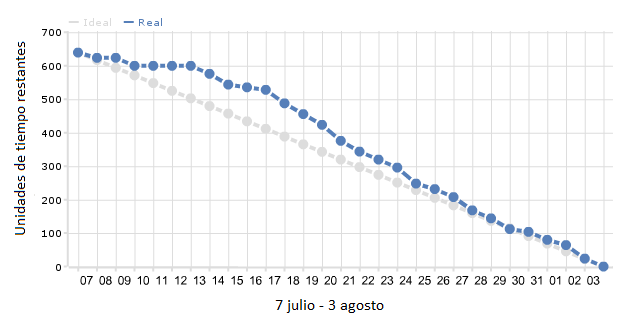
\includegraphics[width=12cm,height=6cm]{figuras/burndown.png}
\caption{Ejemplo gráfico Burn-Down.}
\label{fig:burndown}
\end{figure}

\noindent
\textbf{Gráfico \textit{Burn-Down}}
Herramienta para gestionar y seguir el trabajo de cada sprint, donde se representa gráficamente del avance del sprint. En la figura \ref{fig:burndown} podemos ver este gráfico a modo de ilustración.

\noindent
Las \textbf{modificaciones realizas} sobre la metodología Scrum para realizar este proyecto son dos: 
\begin{itemize}
\item Los roles de \textit{Product Owner} y \textit{Scrum Master} en este proyecto son los mismos, es decir, corresponden a los directores del proyecto, que hacen de voz representativa del cliente y garantizan que se aplique correctamente la metodología. Además, el equipo de desarrollo está representado por una persona.
\item No se realizan las reuniones de monitorización o seguimiento del sprint, ya que en este caso no es necesario realizar un seguimiento tan exhaustivo en el desarrollo y por lo sólo se llevan a cabo cuando existe algún impedimento para continuar con el sprint. Sí se realizan las reuniones de planificación y de revisión del sprint.
\end{itemize}

\noindent
La razón principal de la elección de esta metodología es su flexibilidad a la hora de realizar las diferentes tareas del proyecto, pudiendo seleccionar aquellas tareas que más convienen hacer en un momento dado (las tareas de mayor importancia al principio, para presentar versiones utilizables lo antes posible). Además, en este proyecto existe cierta incertidumbre a la hora de establecer requisitos fijos de antemano, como se puede ver en la sección \ref{riesgos} en el riesgo \textbf{RPD-1}. Así, se desarrollan tareas en función de las necesidades cambiantes durante todo el proyecto y el solapamiento de fases ilustrado en la figura \ref{fig:ciclos} evita que no se tenga que esperar a la finalización de una fase para poder comenzar otra (una de las desventajas de las metodologías pesadas). Otra razón por la que se eligió esta metodología es por la necesidad de ir presentando periódicamente versiones utilizables de la aplicación al cliente (los directores), para que éstos puedan empezar a utilizar la aplicación desde el principio e ir sugiriendo cambios y mejoras a realizar (característica de entornos con incertidumbre). Por ello, las reuniones de planificación y revisión de los sprints (incrementos) son tan importantes en este proyecto.

\section{Gestión de la configuración}
La configuración del software es el conjunto de características funcionales y físicas del software detalladas en la documentación técnica o alcanzadas en un producto. (IEEE610.12-90). La gestión de la configuración, por su parte, es un proceso cuyo propósito es establecer y mantener la integridad de los elementos de trabajo. Para ello, se identifican los elementos y se controlan los cambios de éstos a lo largo de su ciclo de vida, registrando el estado y verificando que estén completos y que sean los correctos.

Para llevar a cabo la gestión de la configuración en este proyecto, se utiliza un sistema de control de versiones mediante la herramienta GitLab que ofrece el CiTIUS y que facilita la gestión de repositorios. Esta herramienta, se basa en GIT, que es un SCV (sistema de control de versiones) multiplataforma y distribuido, donde hay un repositorio central con el cual se puede sincronizar todo el mundo. Se sitúa en una máquina en concreto y es el repositorio que contiene todo el histórico, etiquetas y ramas. La razón de utilizar esta herramienta es su velocidad, su diseño sencillo y la posibilidad de visualizar gráficamente la interacción (gráficas de modificaciones, etc.) con el repositorio.

\noindent
En este proyecto los elementos de configuración implican tanto los archivos de desarrollo como los archivos de documentación:
\begin{itemize}
\item Módulo de Python de los tests estadísticos (paramétricos y no paramétricos).
\item API REST.
\item Archivos de la web: archivos HTML, CSS, JavaScript, imágenes, etc.
\item Memoria.
\item Documentación del módulo de Python de los tests estadísticos.
\end{itemize}

\noindent
El proceso de gestión de configuración es el siguiente:
\begin{enumerate}
\item Se dispone de una rama principal denominada \textit{master} que hace la labor de \textbf{línea base} (donde se encuentran los archivos de los sprints finalizados, es decir, los archivos con los cambios del último sprint).
\item Para mantener organizada y de forma accesible la información, cada sprint se realiza en una rama de desarrollo separada de la rama \textit{master}. Cuando se finaliza el sprint se fusiona en la rama principal.

- La nomenclatura de las ramas será la siguiente: ``sprintX", donde X representa el número de sprints actual.

- En la rama de desarrollo del sprint se van realizando los cambios a los archivos, indicando con una breve descripción los cambios que se hacen.
\item Al finalizar cada sprint, también se crea una etiqueta o \textit{tag} de la rama de desarrollo para tener disponibles todas las versiones de la aplicación (todos los sprints) en un archivo comprimido.

- La nomenclatura de las etiquetas será la siguiente: ``v0.X", donde X representa el número de sprints actual.
\end{enumerate}

\section{Planificación temporal}

\section{Estimación de costes}